\documentclass{letter}
\usepackage{geometry}
\geometry{a4paper, top=1.5cm, left=1.5cm, bottom=1.5cm, right=1.5cm}
\usepackage{hyperref}
\usepackage{nopageno}
\usepackage{graphicx}
\usepackage{wrapfig}
\usepackage{setspace}
\usepackage{color}
\usepackage{calligra}
\usepackage[T1]{fontenc}
\usepackage{xepersian}
\settextfont{XB Niloofar}
\defpersianfont\nastaliq[Scale=1.7]{IranNastaliq}
\begin{document}
%%%%%%%%%%%%%%%%%%%%%%%%%%%%%5
%%%%%%%%%%%%%%%%%%%%%%%%%%%%%
%%%%%%%%%%%%%%%%%%%%%%%%%%%%%%%%%%
%%%%%%%%%%%%% PREAMBLE %%%%%%%%%%%
%%%%%%%%%%%%%%%%%%%%%%%%%%%%%%%%
%%%%%%%%%%%%%%%%%%%%%%%%%%%%%%%%%
%%%%%%%%%%%%%%%%%%%%%%%%%%%%%%%%%%%%
\begin{large}
\textbf{{\nastaliq پوریا چراغی}} \hskip 10.2cm  \textbf{\lr{{\calligra \huge Pooryaa Cheraaqee}}}

	{\nastaliq پژوهشگر حوزه‌ی بینایی ماشین} \hskip 4.9cm  \textbf{\lr{{\calligra \huge Computer Vision Researcher}}}
\end{large}
\vskip 0.02cm
رایانامه: \lr{\texttt{p.cheraaghi@gmail.com}} \hskip 8cm \lr{e-mail:\texttt{p.cheraaghi@gmail.com}}

تلفن: ۶۷۵-۰-۴۲۵-۰۹۳۹ \hskip 10.5cm \lr{phone: +98-9394250675}

تارنما:\href{https://scholar.google.com/citations?user=ebSTTkAAAAAJ&hl=en&oi=ao}{گوگل اسکولار}، \href{https://github.com/cheraaqee}{گیت‌هاب} \hskip 8.5cm \lr{on the web:\href{https://scholar.google.com/citations?user=ebSTTkAAAAAJ&hl=en&oi=ao}{Google Scholar}, \href{https://github.com/cheraaqee}{Git-Hub}}

متولد ۱۰ فروردین ۱۳۷۱ \hskip 11cm \lr{Born on March 30th, 1992}

%%%%%%%%%%%%%%%%%%%%%%%%%%%%%%%%%%%%%%%%%%%%%%%%%%%%%%%%%%%
%%%%%%%%%%%%%%%%%%%%%%%%%%%%%%%%%%%%%%%%%%%%%%%%%%%%%%%%5
%%%%%%%%%%%%%%%%%%%%%%EDUCATION%%%%%%%%%%%%%%%%%%%%%%%%%%%%
%%%%%%%%%%%%%%%%%%%%%%%%%%%%%%%%%%%%%%%%%%%%%%%%%%%%%%%%%%%
%%%%%%%%%%%%%%%%%%%%%%%%%%%%%%%%%%%%%%%%%%%%%%%%%%%%%%%%%%%
\noindent \rule{18cm}{3pt}

\begin{Large}
	\textbf{تحصیلات}\hskip 13.5cm \lr{\textbf{Education}}
\end{Large}

\textbf{کارشناسی ارشد مهندسی کامپیوتر}\hskip 9.7cm \lr{\textbf{MSc Computer Science}}

گرایش هوش مصنوعی و رباتیکز \hskip 9cm {\lr{Artificial Intelligence and Robotics}}

\href{https://khu.ac.ir}{دانشگاه خوارزمی}، ۱۳۹۵-۱۳۹۸ \hskip 9cm \lr{\href{https://khu.ac.ir/en}{Kharazmi University}, 2016-2019}

موضوع پایان‌نامه:\hskip 15cm Thesis:

\href{https://ganj.irandoc.ac.ir/#/articles/815c4b4b589480a070f023280771c679}{ارزیابی کیفیّت تصاویر با تخریب چندگانه} \hskip 1cm \emph{\lr{A No-Reference Method for Assessing the Quality of Multiply Distorted Images}}

%%%%%%%%%%%%%%%%%%%%%%%%%%%%%%%%%%%%%%%%%%%%%%%%%%%%%%%%5
%%%%%%%%%%%%%%%%%%%%%%%%%%%%%%%%%%%%%%%%%%%%%%%%%%%%%%
%%%%%%%%%%%%%%%%%%%%%% PUBLICATIONS %%%%%%%%%%%%%%%%%%%%5
%%%%%%%%%%%%%%%%%%%%%%%%%%%%%%%%%%%%%%%%%%%%%%%%%%%%%%%%%%
%%%%%%%%%%%%%%%%%%%%%%%%%%%%%%%%%%%%%%%%%%%%%%%%%%%
\noindent \rule{18cm}{3pt}

\begin{Large}
	\textbf{مقالات}\hskip 13.5cm \lr{\textbf{Publications}}
\end{Large}

\begin{latin}
	- Cheraaqee, Pooryaa, Zahra Maviz, Azadeh Mansouri, and Ahmad Mahmoudi-Aznaveh. \textbf{``Quality Assessment of Screen Content Images in Wavelet Domain."} IEEE Transactions on Circuits and Systems for Video Technology (2021).

	- Heydari, Maryam, Pooryaa Cheraaqee, Azadeh Mansouri, and Ahmad Mahmoudi-Aznaveh. \textbf{``A low complexity wavelet-based blind image quality evaluator."} Signal Processing: Image Communication 74 (2019): 280-288.

	- Cheraaqee, Pooryaa, Azadeh Mansouri, and Ahmad Mahmoudi-Aznaveh. \textbf{``Incorporating Gradient Direction for Assessing Multiple Distortions."} In 2019 4th International Conference on Pattern Recognition and Image Analysis (IPRIA), pp. 109-113. IEEE, 2019.

	- Motamednia, Hossein, Pooryaa Cheraaqee, and Azadeh Mansouri. \textbf{``Exploring the Gradient for Video Quality Assessment."} In 2020 International Conference on Machine Vision and Image Processing (MVIP), pp. 1-7. IEEE, 2020.

	- Motamednia, Hossein, Mohammad Minouei, Pooryaa Cheraaqee, and Mohammad Reza Soheili. \textbf{``High-Resolution Document Image Reconstruction from Video."} In 2020 International Conference on Machine Vision and Image Processing (MVIP), pp. 1-7. IEEE, 2020.

	- Arezoomand, Amirhoessein, Pooryaa Cheraaqee, Azadeh Mansouri. \textbf{Perceptually Optimized Loss Function for Image Super-Resolution} Submitted to 2021 7th International Conference on Signal Processing and Intelligent Systems, IEEE \href{https://github.com/cheraaqee/popSR/}{https://github.com/cheraaqee/popSR/}
\end{latin}
%%%%%%%%%%%%%%%%%%%%%%%%%%%%%%%%%%%%%%%%%%%%%%%%%%%%%%%%5
%%%%%%%%%%%%%%%%%%%%%%%%%%%%%%%%%%%%%%%%%%%%%%%%%%%%%%
%%%%%%%%%%%%%%%%%%%%%% SKILLs  %%%%%%%%%%%%%%%%%%%%5
%%%%%%%%%%%%%%%%%%%%%%%%%%%%%%%%%%%%%%%%%%%%%%%%%%%%%%%%%%
%%%%%%%%%%%%%%%%%%%%%%%%%%%%%%%%%%%%%%%%%%%%%%%%%%%
\noindent \rule{18cm}{3pt}

\begin{Large}
	\textbf{مهارت‌ها}\hskip 15cm \lr{\textbf{Skills}}
\end{Large}

\textbf{- ارائه و انتقال مفاهیم} \hskip 8.5cm \lr{\textbf{- Presenting and Explaining Concepts}}

کاربر حرفه‌ای \LaTeX \hskip 11.8cm \lr{Professional \LaTeX~user}

\textbf{- برنامه‌نویسی}\hskip 13.4cm \lr{\textbf{- Programming}}

پایتون و متلب (کاربر عادی)، \lr{C/C++} (مبتدی) \hskip 3.6cm \lr{Python, MATLAB (regular user), C/C++ (beginner)}

\textbf{- سیستم عامل} \hskip 12.4cm \textbf{\lr{- Operating System}}

کاربر عادی لینوکس \hskip 12.4cm \lr{Regular Linux user}

\textbf{- انگلیسی} \hskip 14.8cm \lr{\textbf{- English}}

مسلّط به خواندن، نوشتن و گفت و گو \hskip 10.6cm \lr{Professional user}

\textbf{- شبکه‌های عصبی و یادگیری ماشین} \hskip 6cm \textbf{\lr{- Neural Networks and Machine Learning}}

\lr{keras}، \lr{SciKit-Learn} و \lr{LibSVM} \hskip 8cm \lr{Keras, SciKit-Learn,  and LibSVM}

\textbf{- پردازش تصویر}\hskip 12.5cm\lr{\textbf{- Image Processing}}

جعبه‌ابزار پردازش تصویر متلب و کتابخانه‌ی \lr{OpenCV-Python}\hskip 3.3cm \lr{MATLAB IP toolbox and OpenCV-Python}

\textbf{- کار تیمی} \hskip 14.3cm \lr{\textbf{- Teamwork}}

کاربر عادی Git \hskip 13.3cm \lr{Regular Git user}

\textbf{- ریاضیات} \hskip 15.1cm \lr{\textbf{- Math}}

قادر به مدل کردن مسائل مختلف با مفاهیم ریاضی \hskip 1.2cm \lr{Capable of modeling real-world problems with mathematical concepts}
%%%%%%%%%%%%%%%%%%%%%%%%%%%%%%%%%%%%%%%%%%%%%%%%%%%%%%%%5
%%%%%%%%%%%%%%%%%%%%%%%%%%%%%%%%%%%%%%%%%%%%%%%%%%%%%%
%%%%%%%%%%%%%%%%%%%%%% EXPERIENCES  %%%%%%%%%%%%%%%%%%%%5
%%%%%%%%%%%%%%%%%%%%%%%%%%%%%%%%%%%%%%%%%%%%%%%%%%%%%%%%%%
%%%%%%%%%%%%%%%%%%%%%%%%%%%%%%%%%%%%%%%%%%%%%%%%%%%

\noindent \rule{18cm}{3pt}

\begin{Large}
	\textbf{تجارب}\hskip 13.6cm \lr{\textbf{Experiences}}
\end{Large}

\textbf{- مترجم}\hskip 15cm \lr{\textbf{- Translator}}

 مؤسّسه‌ی چاپ الکترونیک \href{https://instagram.com/nashrafa}{نشرآفا}، تابستان ۱۳۹۷-بهار ۱۳۹۸ \hskip 1cm \lr{\href{https://instagram.com/nashrafa}{Nashrafa} On-Line Publishing Co., Summer 2019- Spring 2020}

\textbf{- تدریس} \hskip 14.5cm \textbf{\lr{- Instructor}}

آزمایشگاه سیستم عامل- \href{https://ce.guilan.ac.ir}{دانشگاه گیلان}، پائیز ۹۸ \hskip 5.6cm \lr{O.S. Lab, \href{https://guilan.ac.ir/en/home}{University of Guilan}, Fall 2019}

حلّ تمرین معماری کامپیوتر- \href{https://guilan.ac.ir/staff?p_p_auth=xGJ4TC4g&p_p_id=eduteacherdisplay_WAR_edumanagerportlet&p_p_lifecycle=0&p_p_state=normal&p_p_mode=view&p_p_col_id=_118_INSTANCE_P4x3SQKwRDdD__multitab-1&p_p_col_count=1&_eduteacherdisplay_WAR_edumanagerportlet_mvcPath=\%2Fedu-teacher-display\%2Fdisplay\%2Fsimple.jsp&_eduteacherdisplay_WAR_edumanagerportlet_teacherId=2476030&_eduteacherdisplay_WAR_edumanagerportlet_tabs1=offered-lessons&_eduteacherdisplay_WAR_edumanagerportlet_delta=20&_eduteacherdisplay_WAR_edumanagerportlet_keywords=&_eduteacherdisplay_WAR_edumanagerportlet_advancedSearch=false&_eduteacherdisplay_WAR_edumanagerportlet_andOperator=true&_eduteacherdisplay_WAR_edumanagerportlet_name=&_eduteacherdisplay_WAR_edumanagerportlet_nowTab=&_eduteacherdisplay_WAR_edumanagerportlet_resetCur=false&cur=2}{استاد احمدی‌فر}، پائیز ۹۳- تابستان ۹۴\hskip 0.7cm \lr{T.A. for Computer Architecture Course- \href{https://scholar.google.com/citations?user=WT1Jve8AAAAJ&hl=en}{Prof. Ahmadifar}}

حلّ تمرین طراحی الگوریتم- \href{https://www.linkedin.com/in/shahram-moadab-94b79253/?originalSubdomain=ir}{استاد مؤدّب}، پائیز ۹۳-تابستان ۹۴\hskip 2.5cm \lr{T.A. for Algorithm Design Course- \href{https://www.linkedin.com/in/shahram-moadab-94b79253/?originalSubdomain=ir}{Prof. Moadab}}

حلّ تمرین شبکه‌های عصبی- \href{https://khu.ac.ir/cv/307/\%D8\%A2\%D8\%B2\%D8\%A7\%D8\%AF\%D9\%87\%20\%D9\%85\%D9\%86\%D8\%B5\%D9\%88\%D8\%B1\%DB\%8C}{استاد منصوری}- اکنون \hskip 2.25cm \lr{T.A. for Neural Networks Course- \href{https://scholar.google.com/citations?user=eK03yPgAAAAJ}{Prof. Mansouri}- Current}

\textbf{- پروژه}\hskip 15cm {\lr{\textbf{- Projects}}

ارزیابی کیفیت تصاویر نمامفاد- نهاد ریاست جمهوری \lr{Quality Assessment of Screen Content-Iran National Science Foundation}

شناسایی چهره در تصویر- آزاد \hskip 5.5cm\lr{Face Recognition with Deep Learning, As a free-lancer}

شناسایی اشیاء در تصویر- آزاد \hskip 3.6cm\lr{Customized Object Detection with Deep Learning, As a free-lancer}
%%%%%%%%%%%%%%%%%%%%%%%%%%%%%%%%%%%%%%%%%%%%%%%%%%%%%%%%5
%%%%%%%%%%%%%%%%%%%%%%%%%%%%%%%%%%%%%%%%%%%%%%%%%%%%%%
%%%%%%%%%%%%%%%%%%%%%% INTERESTS  %%%%%%%%%%%%%%%%%%%%5
%%%%%%%%%%%%%%%%%%%%%%%%%%%%%%%%%%%%%%%%%%%%%%%%%%%%%%%%%%
%%%%%%%%%%%%%%%%%%%%%%%%%%%%%%%%%%%%%%%%%%%%%%%%%%%

\noindent \rule{18cm}{3pt}

\begin{Large}
	\textbf{\textcolor{blue}{علایق}}
\end{Large}

\textcolor{blue}{ریاضیّات گسسته، شبیه‌سازی کامپیوتری، مصوّرسازی داده، سیستم بینایی انسان، فشرده‌سازی داده، طرّاحی، خوشنویسی، تکواندو، فیزیک، زبان، ادبیّات، پویانمایی و سینما}

\begin{latin}
\begin{Large}
	\textcolor{blue}{\lr{\textbf{ّInterests}}}
\end{Large}

	\textcolor{blue}{Discrete Mathematics, Computer Simulation, Data Visualization, Human Visual System, Data Compression, Graphics, Calligraphy, Taekwondo, Physics, Language, Literature, Annimation, and Movies.}
\end{latin}
\vskip 1cm
\begin{LTR}
	\hskip 0.5cm 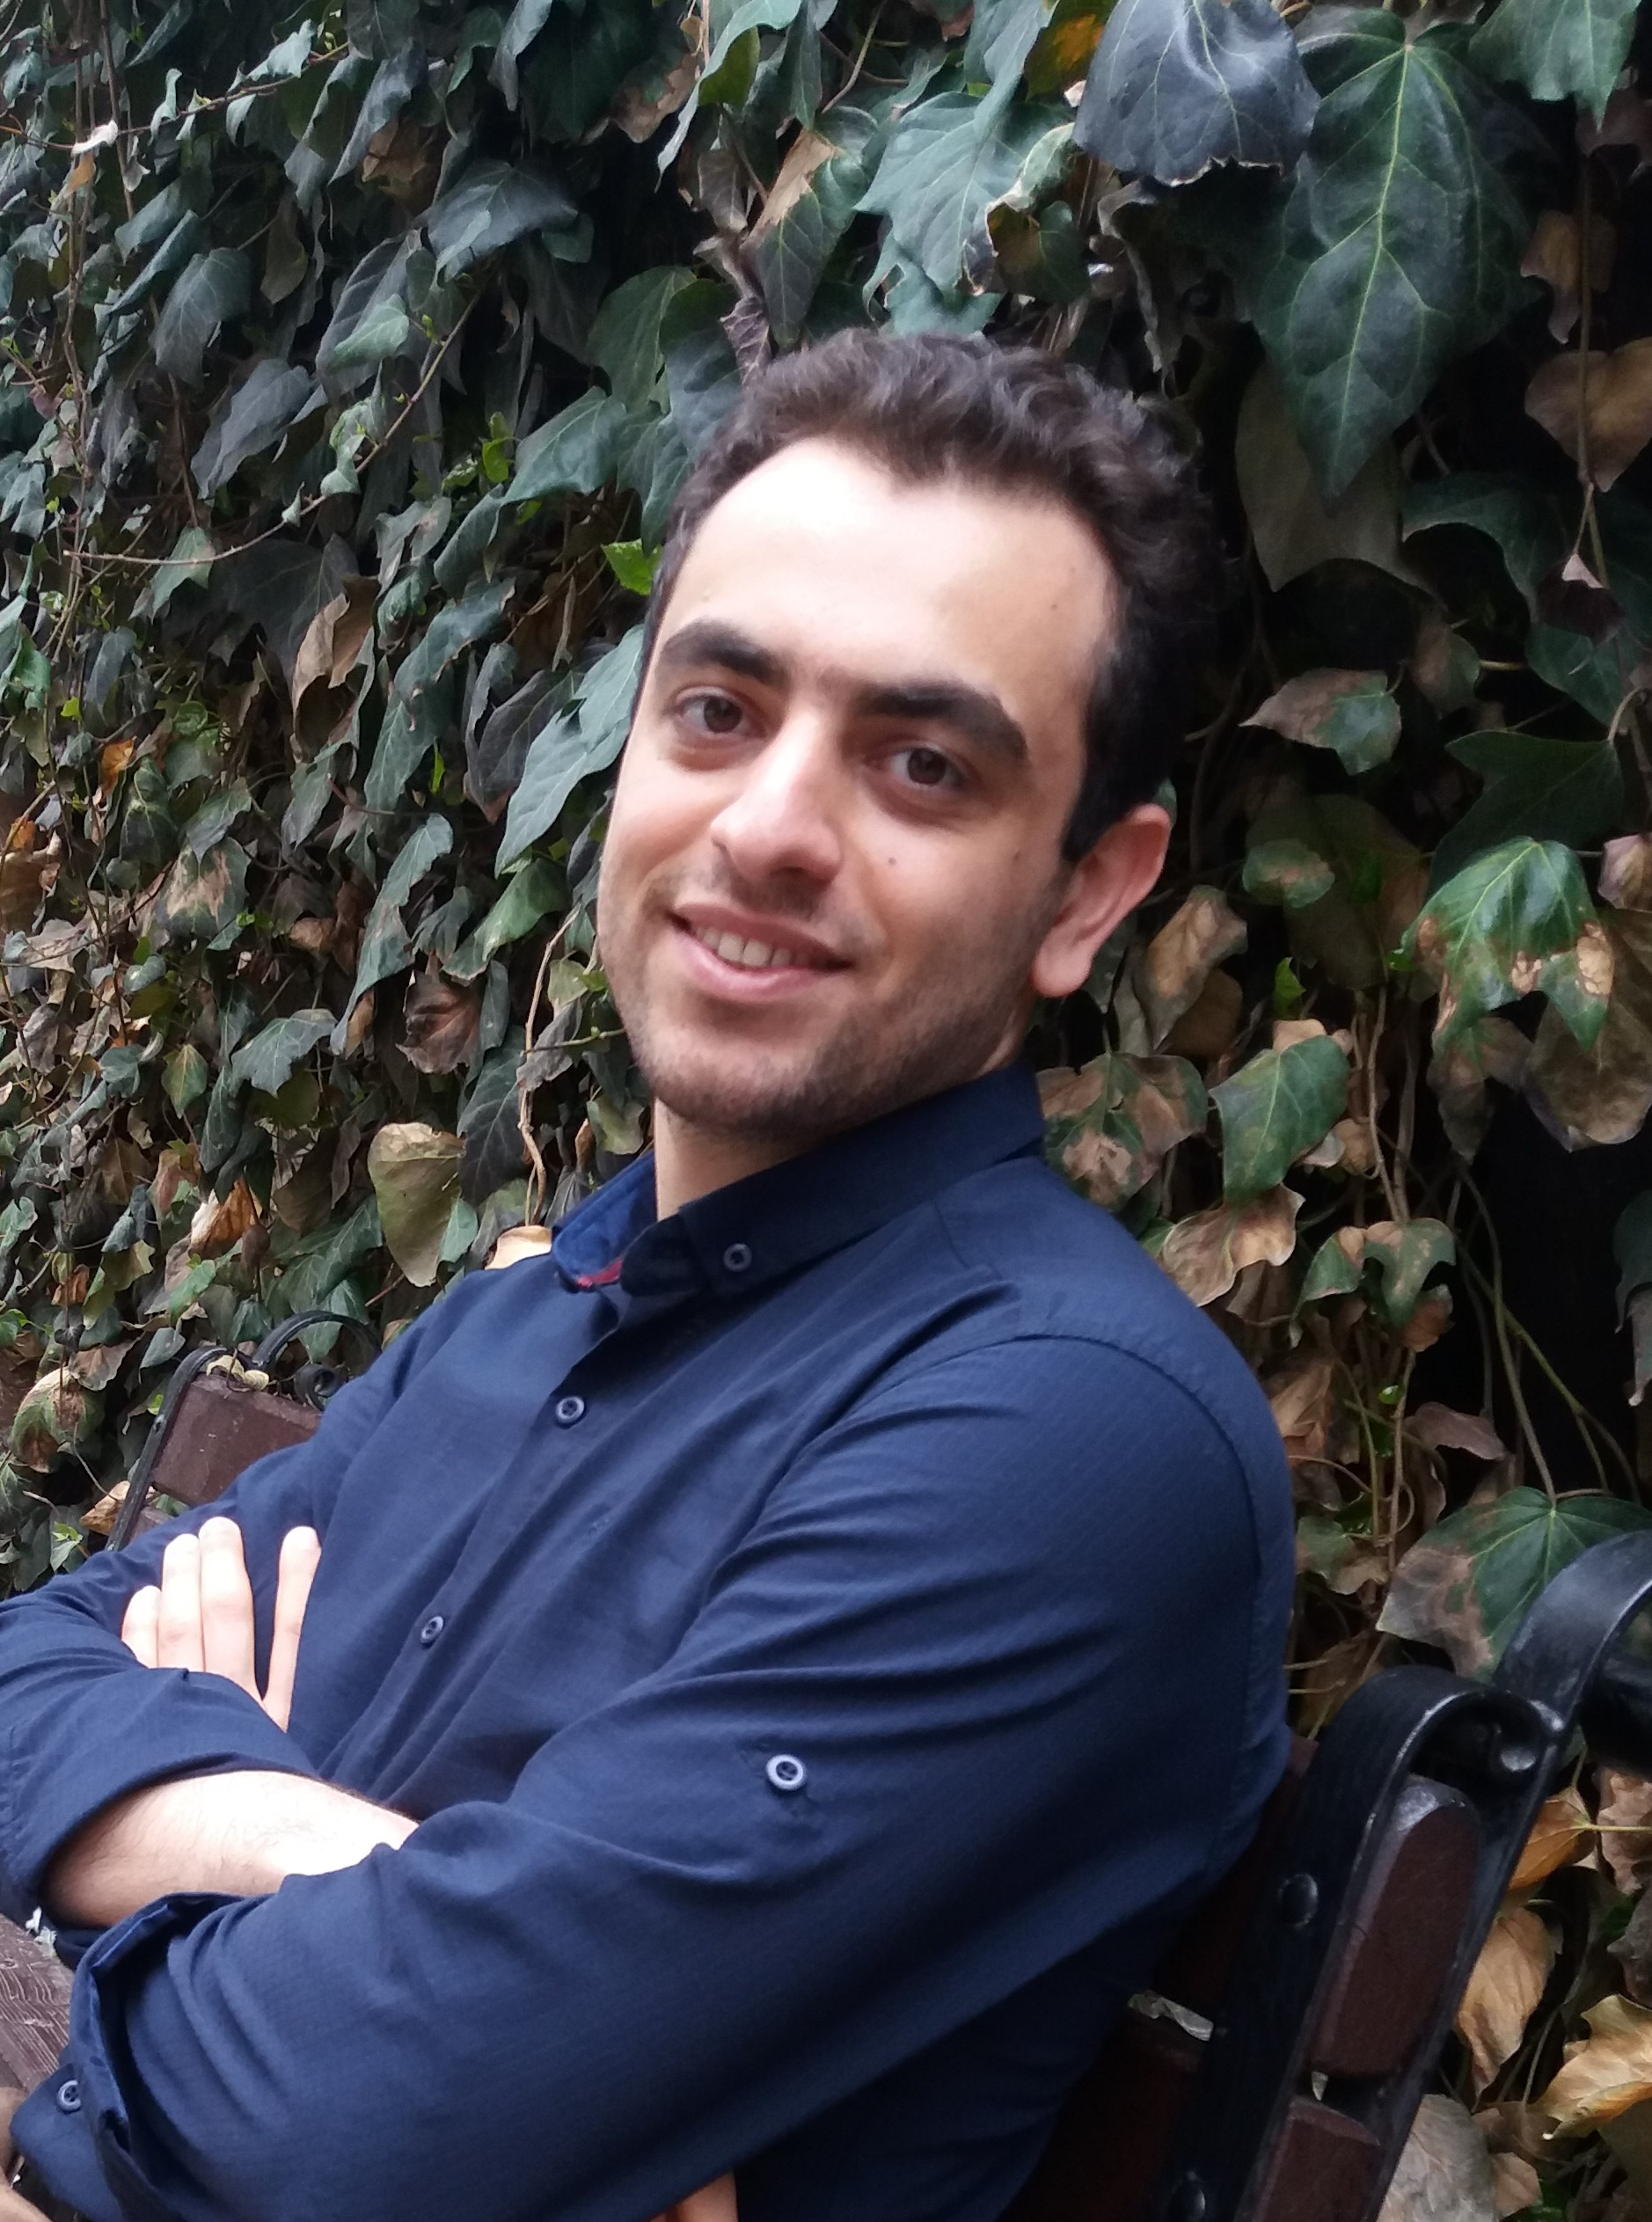
\includegraphics[trim={13cm 20cm 10cm 10cm}, clip, height=6cm]{../profile_pic}
\end{LTR}
\end{document}
